\documentclass[border=10pt]{standalone}
\usepackage{tikz}
\usetikzlibrary{automata, positioning, arrows.meta}

\begin{document}
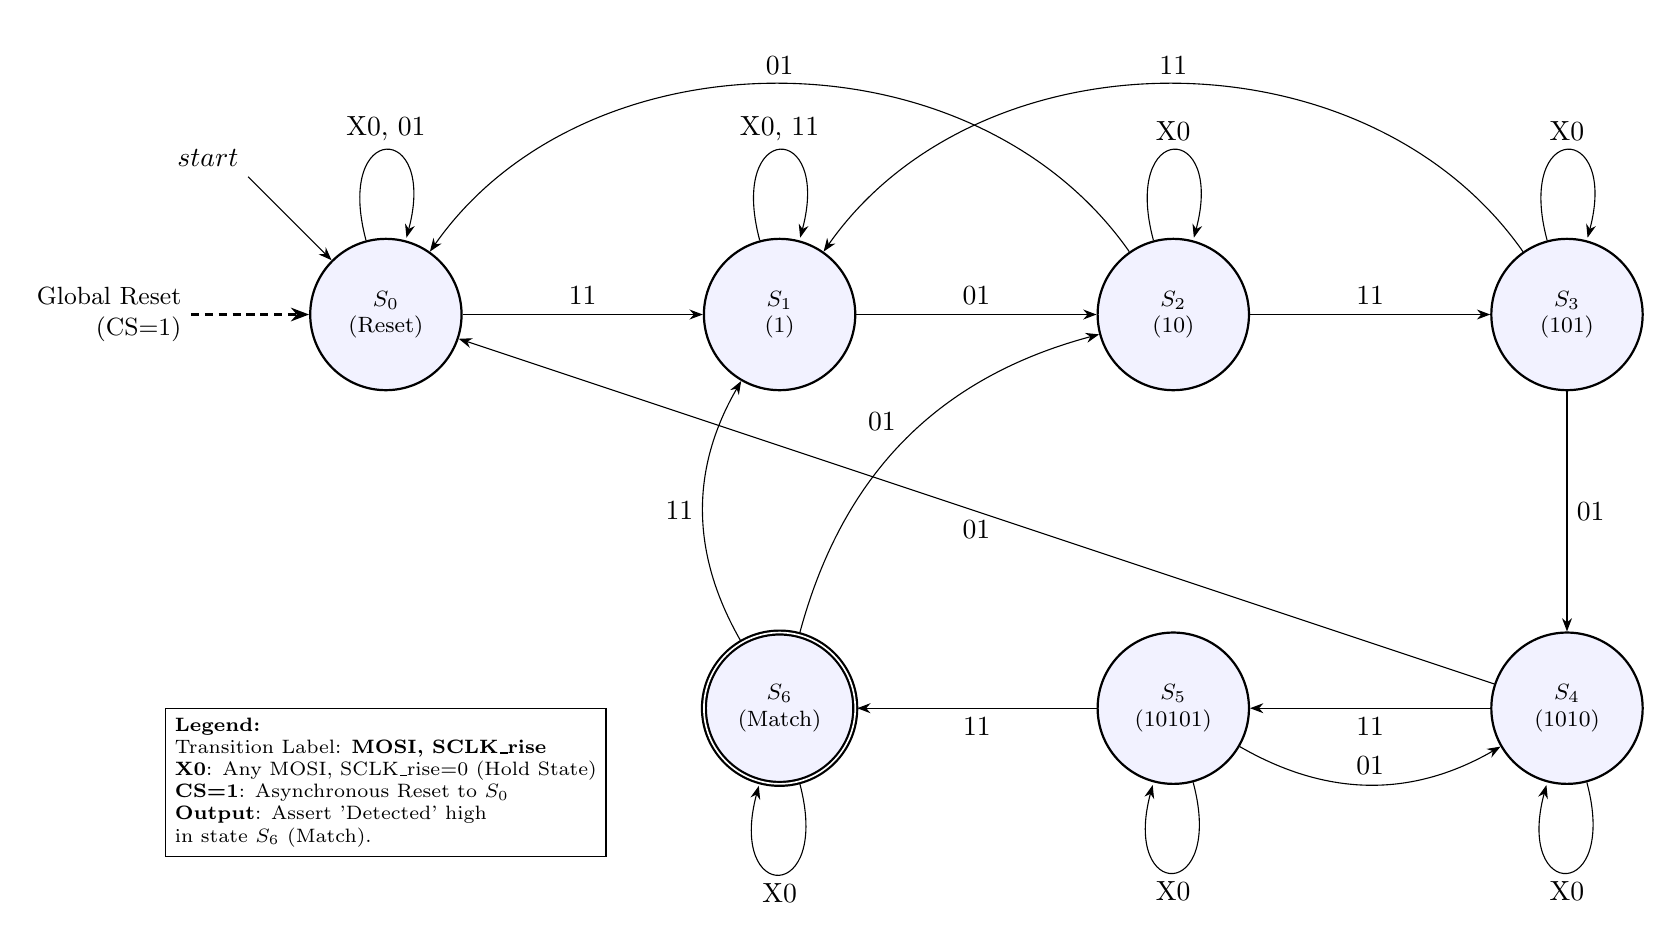
\begin{tikzpicture}[
    ->, >=Stealth, auto, node distance=5cm,
    every state/.style={thick, fill=blue!5, text width=1.5cm, align=center, font=\footnotesize},
    initial text=$start$
]

    % Sequence: 101011
    % Inputs: MOSI, SCLK_rise
    % Hold on SCLK_rise=0 (X0)
    % Transition on SCLK_rise=1 (X1)
    
    % States
    \node[state] (s0) {$S_0$\\ (Reset)};
    
    % Manual Start Arrow at 135 degrees
    \draw [<-] (s0.135) -- ++(135:1.5cm) node [anchor=south east] {$start$};

    \node[state, right of=s0] (s1) {$S_1$\\ (1)};
    \node[state, right of=s1] (s2) {$S_2$\\ (10)};
    \node[state, right of=s2] (s3) {$S_3$\\ (101)};
    \node[state, below of=s3] (s4) {$S_4$\\ (1010)};
    \node[state, left of=s4] (s5) {$S_5$\\ (10101)};
    \node[state, left of=s5, accepting] (s6) {$S_6$\\ (Match)};

    % Transitions for Sequence 101011
    % Labels: MOSI, SCLK_rise
    
    % S0: Start
    % S0: Start
    \node[left=1.5cm of s0, font=\small, align=right] (reset) {Global Reset\\(CS=1)};
    \draw[->, densely dashed, thick] (reset) -- (s0);

    \path (s0) edge[loop above] node {X0, 01} (s0) % Hold or MOSI=0,SCLK_rise=1
               edge node {11} (s1); % MOSI=1, SCLK_rise=1
               
    % S1: Got 1
    \path (s1) edge[loop above] node {X0, 11} (s1) % Hold or Stay on 1
               edge node {01} (s2); % Next 0
               
    % S2: Got 10
    \path (s2) edge node {11} (s3) % Next 1
               edge[loop above] node {X0} (s2) % Hold
               edge[bend right=55] node[above] {01} (s0); % Reset on 0
    
    % S3: Got 101
    \path (s3) edge node {01} (s4) % Next 0
               edge[loop above] node {X0} (s3) % Hold
               edge[bend right=55] node[above] {11} (s1); % Back to S1 on 1
               
    % S4: Got 1010
    \path (s4) edge node {11} (s5) % Next 1
               edge[loop below] node {X0} (s4) % Hold
               edge node[below] {01} (s0); % Reset
               
    % S5: Got 10101
    \path (s5) edge node {11} (s6) % Next 1 -> Match
               edge[loop below] node {X0} (s5) % Hold
               edge[bend right] node {01} (s4); % Back to S4 (1010 on 0)
               
    % S6: Match (101011).
    \path (s6) edge[loop below] node {X0} (s6) % Hold
               edge[bend left] node {11} (s1)
               edge[bend left] node {01} (s2);

    % Legend
    \node[draw, rectangle, fill=white, align=left, font=\scriptsize, anchor=north] at (0,-5) (legend) {
        \textbf{Legend:} \\
        Transition Label: \textbf{MOSI, SCLK\_rise} \\
        \textbf{X0}: Any MOSI, SCLK\_rise=0 (Hold State) \\
        \textbf{CS=1}: Asynchronous Reset to $S_0$ \\
        \textbf{Output}: Assert 'Detected' high \\
        in state $S_6$ (Match).
    };

\end{tikzpicture}
\end{document}
